\documentclass[a4paper,twoside]{article}
\usepackage[T1]{fontenc}
\usepackage[bahasa]{babel}
\usepackage{graphicx}
\usepackage{graphics}
\usepackage{float}
\usepackage[cm]{fullpage}
\pagestyle{myheadings}
\usepackage{etoolbox}
\usepackage{setspace} 
\usepackage{lipsum} 
\setlength{\headsep}{30pt}
\usepackage[inner=2cm,outer=2.5cm,top=2.5cm,bottom=2cm]{geometry} %margin
% \pagestyle{empty}

\graphicspath{{./Gambar/}}% folder tempat gambar 

\makeatletter
\renewcommand{\@maketitle} {\begin{center} {\LARGE \textbf{ \textsc{\@title}} \par} \bigskip {\large \textbf{\textsc{\@author}} }\end{center} }
\renewcommand{\thispagestyle}[1]{}
\markright{\textbf{\textsc{Laporan Perkembangan Pengerjaan Skripsi\textemdash Sem. Genap 2015/2016}}}

\onehalfspacing
 
\begin{document}

\title{\@judultopik}
\author{\nama \textendash \@npm} 

%ISILAH DATA BERIKUT INI:
\newcommand{\nama}{Gabriel Panji Lazuardi}
\newcommand{\@npm}{2016730068}
\newcommand{\tanggal}{01/12/2021} %Tanggal pembuatan dokumen
\newcommand{\@judultopik}{Aplikasi mobile IDE UNPAR berbasis Moodle App} % Judul/topik anda
\newcommand{\kodetopik}{PAN4902}
\newcommand{\jumpemb}{1} % Jumlah pembimbing, 1 atau 2
\newcommand{\pembA}{Pascal Alfadian}
\newcommand{\pembB}{-}
\newcommand{\semesterPertama}{49 - Ganjil 20/21} % semester pertama kali topik diambil, angka 1 dimulai dari sem Ganjil 96/97
\newcommand{\lamaSkripsi}{1} % Jumlah semester untuk mengerjakan skripsi s.d. dokumen ini dibuat
\newcommand{\kulPertama}{Skripsi 1} % Kuliah dimana topik ini diambil pertama kali
\newcommand{\tipePR}{B} % tipe progress report :
% A : dokumen pendukung untuk pengambilan ke-2 di Skripsi 1
% B : dokumen untuk reviewer pada presentasi dan review Skripsi 1
% C : dokumen pendukung untuk pengambilan ke-2 di Skripsi 2

% Dokumen hasil template ini harus dicetak bolak-balik !!!!

\maketitle

\pagenumbering{arabic}

\section{Data Skripsi} %TIDAK PERLU MENGUBAH BAGIAN INI !!!
Pembimbing utama/tunggal: {\bf \pembA}\\
Pembimbing pendamping: {\bf \pembB}\\
Kode Topik : {\bf \kodetopik}\\
Topik ini sudah dikerjakan selama : {\bf \lamaSkripsi} semester\\
Pengambilan pertama kali topik ini pada : Semester {\bf \semesterPertama} \\
Pengambilan pertama kali topik ini di kuliah : {\bf \kulPertama} \\
Tipe Laporan : {\bf \tipePR} -
\ifdefstring{\tipePR}{A}{
			Dokumen pendukung untuk {\BF pengambilan ke-2 di Skripsi 1} }
		{
		\ifdefstring{\tipePR}{B} {
				Dokumen untuk reviewer pada presentasi dan {\bf review Skripsi 1}}
			{	Dokumen pendukung untuk {\bf pengambilan ke-2 di Skripsi 2}}
		}
		
\section{Latar Belakang}
IDE UNPAR adalah \textit{learning management system} berbasis web yang digunakan oleh UNPAR untuk membantu proses pembelajaran interaktif. IDE UNPAR bekerja dengan menyediakan mata kuliah yang diambil oleh mahasiswa secara virtual lengkap dengan peserta lain dari mata kuliah tersebut yang dapat mengaksesnya. IDE UNPAR juga membantu dosen merencanakan dan memantau proses pembelajaran. Mahasiswa juga dipermudah untuk melihat dan mengetahui proses dan tujuan pembelajaran dari suatu mata kuliah. 

Berdasarkan footer pada IDE UNPARR, IDE UNPAR dibuat dengan menggunakan \textit{Blackboard Open Learning Management System}\cite{IDEUNPAR} yang merupakan program berbasis Moodle, namun berdasarkan halaman bantuan \textit{Blackboard Open Learning Management System}, \textit{Blackboard Open Learning Management System} telah berganti menjadi \textit{Open LMS}\cite{Blackboard},sehingga penelitian ini akan befokus kepada Moodle. Moodle adalah \textit{learning management system} bersifat \textit{Open-source} yang dibuat menggunakan bahasa pemrograman \textit{PHP}. Moodle dilisensikan dibawah lisensi \textit{GNU GENERAL PUBLIC LICENSE Version 3, 29 June 2007}. Lisensi tersebut memperbolehkan adannya modifikasi terhadap program yang dilisensikan.

Moodle menyediakan \textit{source code} untuk \textit{learning management system} berbasis mobile. Moodle mobile memungkinkan penggunanya mengakses \textit{learning management system} berbasis Moodle web melalui perangkat mobile mereka. Pengguna Moodle mobile dapat mengakses \textit{learning management system} yang mereka gunakan dengan memasukkan \textit{URL} \textit{learning management system} dan memasukkan kredensial login mereka apabila diperlukan. Moodle mobile akan menampilkan data dan memberi akses yang serupa dengan apa yang ada pada \textit{learning management system} Moodle web. Moodle mobile dibangung dengan menggunakan \textit{Ionic Framework}. \textit{Ionic Framework} adalah sebuah \textit{Software development kit} untuk membuat aplikasi mobile dan desktop dengnan menggunakan teknologi seperti HTML, CSS dan \textit{Javascript}\cite{Ionic:intro}. Moodle mobile dilisensikan dibawah lisensi   \textit{APACHE LICENSE, VERSION 2.0}. Lisensi tersebut juga memperbolehkan dilakukannya modidfikasi terhadap \textit{source} dari aplikasi.
\section{Rumusan Masalah}
Rumusan masalah yang akan dibahas dalam penulisan skripsi ini adalah :
\begin{itemize}
	\item Bagaimana Moodle mobile IDE UNPAR dapat mengakses IDE UNPAR?
	\item Perbaikan apa saja yang dapat dilakukan untuk mempermudah penggunaan Moodle mobile?
	\item Bagaimana implementasi perbaikan tersebut ke dalam Moodle mobile?
\end{itemize}
\section{Tujuan}
Tujuan yang ingin dicapai dalam penulisan skripsi ini adalah :
\begin{enumerate}
	\item Menghubungkan Moodle mobile IDE UNPAR dengan Moodle web IDE UNPAR agar data yang ditampilkan sama.
	\item Melakukan \textit{hardcode} URL "https://ide.unpar.ac.id" agar saat aplikasi dibuka pengguna tidak perlu memasukkan alamat IDE UNPAR.
	\item Menganalisis lisensi dari Moodle dan apabila diperbolehkan merubah branding menjadi UNPAR
\end{enumerate}

\section{Detail Perkembangan Pengerjaan Skripsi}
Detail bagian pekerjaan skripsi sesuai dengan rencan kerja/laporan perkembangan terkahir :
	\begin{enumerate}
		\item \textbf{Memplajari Moodle mobile.}\\
		{\bf Status :} Ada sejak rencana kerja skripsi.\\
		{\bf Hasil :} Memplejari Moodle mobile dengan sumber dari dokumentasi resmi Moodle sudah dilakukan dari awal penulisan dokumen skripsi. 
\begin{itemize}
\item \textbf{Sifat dasar} \\
Moodle mobile dikembangkan menggunakan Ionic karena Ionic memungkinkan pengembangan aplikasi yang bersifat \textit{cross-platform}. Sifat \textit{cross-platform} dari Ionic membuat Moodle mobile dengan mudah diterapkan ke berbagai platform dengan hanya satu \textit{codebase}. Pengembangan aplikasi dengan \textit{view} yang besar akan lebih cepat dengan penggembangan \textit{framework} bersifat \textit{cross-platform} dibandingkan dengan pengembangan secara \textit{native}. 

Moodle mobile bersifat modular seperti Moodle berbasis web yang berarti Moodle mobile juga mendukung \textit{themes} dan \textit{plugins}. \textit{Plugin} akan membantu pengembang menambahkan fitur dengan mudah ke dalam aplikasi Moodle mobile. \textit{Themes} memungkinkan pengembang Moodle mobile untuk mengubah gaya dan layout dari aplikasi Moodle mobile sesuai dengan keinginannya. Pada subbab-subbab berikut akan dibahas mengenai fitur-fitur, \textit{plugin}, dan \textit{theme} dari Moodle mobile.

\item \textbf{\textit{Themes} dan \textit{Plugisn}} \\
\textit{Themes} dan \textit{plugins} pada Moodle mobile bekerja berbeda dengan Moodle berbasis web. Perbedaan yang ada dari Moodle berbasis web dengan Moodle mobile diantaranya adalah \textit{themes} dan \textit{plugin}.Pada Moodle mobile sebelum versi 3.5 \textit{themes} yang sudah digunakan pada Moodle web akan secara otomatis digunakan juga pada Moodle mobile. Moodle mobile versi 3.5 dan seterusnya sudah tidak dapat mendukung penggunaan \textit{themes} lagi karena Ionic versi 3 tidak mendukung \textit{customg themes} dari Moodle sebelum versi 3.5.. Sehingga untuk mengubah tampilan dari Moodle mobile adalah dengan mengubah source code Moodle mobile sendiri. Awalnya \textit{plugin} pada Moodle mobile sebelum versi 3.5 dapat bekerja dengan membuat modul Angular atau Ionic lalu menambahkannya pada bagian \textit{plugin} di dalam Moodle mobile. Semenjak Moodle mobile versi 3.5 plugin dapat digunakan tanpa harus membuat modul Angular atau Ionic, pengembang aplikasi cukup membuat template plugin menggunakan PHP dan \textit{markup} Ionic 3.

\item \textbf{Fitur-fitur} \\
\begin{enumerate}
		\item \textit{See your courses at a glance} \\
			Fitur ini akan menampilkan semua \textit{courses} yang sedang di tempuh dalam bentuk \textit{ion-card} di halam utama Moodle mobile. \textit{Courses} yand ditampilkan juga akan dipisah %more explanation here
			dan pengguna juga dapat memfilter \textit{courses} yang ditempuh. Fitur ini juga dapat digunakan di dalam kondisi luring.
		\item \textit{Easily access course content} \\
			Pengguna dapat mengakses konten dari seluruh \textit{courses} yang ditempuh melalui \textit{courses} yang ditampilkan pada halaman utama. Fitur ini dapat digunakan dalam kondisi luring.
		\item \textit{View and access activities which are due} \\
			Fitur ini dapat diakses melalui tab \textit{timeline}. Tab \textit{timeline} akan menunjukkan aktivitas-aktivitas dari \textit{course} yang ditempuh oleh pengguna secara berurut mulai dari tenggat waktu terdekat. Pengguna akan dapat secara langsung mengakses aktivitas-aktivitas yang ditampilkan melalui tab \textit{timeline}. Fitur ini dapat digunakan di dalam kondisi luring.
		\item \textit{Grades and grading} \\
			Moodle mobile akan menyediakan tautan untuk mengakses buku nilai, dan pengajar dapat melihat nilai dari submisi tugas pelajar. Fitur ini dapat digunakan secara luring.
		\item \textit{Grade assignment} \\
			Pengajar dapat memberikan tugas yang mereka berikan melalui Moodle mobile. Fitur ini dapat digunakan secara luring.
		\item \textit{Notes} \\
			Pengajar dapat melihat catatan situs, \textit{courses}, dan catatan pribadi tentang murid mereka. Fitur ini dapat digunakan secara luring.
		\item \textit{Message participants} \\
			Pengguna dapat mengirim pesan pribadi kepada rekan mereka yang menggunakan Moodle atau terdaftar dalam satu \textit{course} yang sama. Fitur ini hanya dapat digunakan secara daring.
		\item \textit{Take quizess on your mobile device} \\
			Pelajar dapat mengerjakan ujian melalui Moodle mobile. Tidak semua ujian dapat dikerjakan melalui Moodle mobile seperti ujian yang membutuhkan \textit{safe browser}, ujian yang memiliki jenis pertanyaan dimana pertanyaa itu hanya dapat dijawab apabila pertanyaan sebelumnya sudah dijawab. Ujian yang menggunakan \textit{plugin} dapat dikerjakan pada Moodle mobile apabila \textit{plugin} tersebut mendukung Moodle mobile.\cite{moodle:39}
			
			Ujian tidak seluruhnya dapat dikerjakan secara luring. Syarat ujian yang dapat dikerjakan diluar luring adalah ujian tanpa batas waktu, pertanyaan ujian berupa umpan balik yang ditangguhkan, tidak ada kebutuhan alamat jaringa. \cite{moodle:39}
	\end{enumerate}


\end{itemize}

%Survei sudah dilakukan sebanyak 3x pada tanggal X, Y dan Z. Pada kunjungan pertama, diperhaitkan denah museum dan dibuat sketsa berdasarkan pengamatan. Pada kunjunga kedua, bertemu dengan bagian humas museum dan berhasil mendapatkan denah serta melakukan wawancara. Hasil wawancara sudah dibuat dan ada softcopy-nya. Pada kunjungan ketiga, secara khusus dilihat perilaku pengunjung. Masih direncakanan 2x kunjungan lagi. Bukti-bukti kunjungan dapat dilihat di lampiran

		\item \textbf{Menganalisis lisensi pada Moodle mobile}\\
		{\bf Status :} Ada sejak rencana kerja.\\
		{\bf Hasil :} Moodle mobile dilisensikan dengan lisensi \textit{Apache 2.0}. Lisensi tersebut mengizinkan untuk melakukan reproduksi dari Moodle mobile dengan atau tanpa modifikasi. Seperti yang disebut pada poin 4 lisesnsi dengan judul \textit{"Redistribution"}, hal-hal tersebut dapat dilakukan apabila memenuhi syarat-syarat yang tertera. Syarat-syarat yang dimaksud adalah :
\begin{itemize}
\item Aplikasi yang dibuat harus disertakan dengan salinan lisensi \textit{Apcahe 2.0}.
\item Seluruh file yang dimodifikasi harus menyertakan pemberitahuan yang jelas bahwa file tersebut sudah dimodifikasi.
\item Seluruh paten, \textit{trademark}, \textit{copyright} dan pemberitahuan atribusi harus disimpan dalam bentuk sumber untuk seluruh aplikasi yang akan didistrubusikan.
\item Apabila aplikasi sumber menyertakan file teks dengan judul \textit{\textbf{NOTICES}}, maka selurh aplikasi yang akan didistribusikan harus menyertakan salinan yang dapat dibaca.
\end{itemize}

		\item \textbf{Menyiapkan lingkungan pengembangan Moodle mobile}\\
		{\bf Status :} Ada sejak rencana kerja.\\
		{\bf Hasil :} Lingkungan pengembangan disiapkan dengan menggunakan spesifikasi :
\begin{enumerate}
	\item \textit{Browser} Chromium.
	\item Git, dengan \textit{fork} yang mengarah kepada \textit{repository} resmi Moodle mobile.
	\item Node.js versi 14.
	\item \textit{Native build tools} Windows.
\end{enumerate} 
		
		\item \textbf{Menghubungkan Moodle mobile dengan IDE UNPAR.}\\
		{\bf Status :} Ada sejak rencana kerja skripsi.\\
		{\bf Hasil :} Moodle mobile memungkinkan untuk mengatur \textit{URL preset} agar saat Moodle mobile dijalnkan, akan langsung diahlikan ke \textit{URL} tersebut. Namun ketika \textit{URL} IDE UNPAR digunakan terdapat \textit{error} dimana variable \texttt{\$urlscheme} memiliki nilai variable yang sudah diubah, dimana seharusnya variable tersebut berisi \texttt{moodlemobile://token=...} melainkan berisi \texttt{ide.unpar.ac.id://token=....}. Mengubah variable \texttt{urlscheme} pada Moodle mobile tetap tidak memungkinkan  IDE UNPAR diakses melalui Moodle mobile. Karena  adanya konfigurasi yang tidak dapat diakses untuk menghubungkan IDE UNPAR maka situs demo akan digunakan.

		\item \textbf{Menyiapkan situs demo pengganti IDE UNPAR}\\
		{\bf Status :} Ditambahkan semester ini.\\
		{\bf Hasil :} Situs demo untuk menggantikan IDE UNPAR dibuat agar Moodle mobile dapat dihubungkan dan diuji coba selama pengembangan. Situs dibuat pada \textit{server} yang dimiliki oleh pembimging dengan alamat moodledemo.pascal.id. Pada situs demo juga akan dilakukan penyesuaian agar situs tersebut meyerupai IDE UNPAR dalam tampilan dan memiliki data sebagian mata kuliah, dosen pada mata kuliah, dan mahasiswa pada mata kulaih tersebut.

		\item \textbf{Menganalisa perbedaan IDE UNPAR dengann Moodle standar untuk diterapkan dalam Moodle mobile}\\
		{\bf Status :} Ditambahkan semester ini.\\
		{\bf Hasil :} Karena IDE UNPAR sudah mengalamai modifikasi maka modifikasi-modifikasi tersebut juga akan diimplementasikan pada Moodle mobile dan situs demo. Modifikasi yang dimaksud adalah : 
\begin{enumerate}
\item \textbf{Penggunaan tema Snap Moodle} \\
	Tampilan IDE UNPAR sudah berbeda dari tampilan standar milik Moodle. perubahan ini terlihat ketika memeriksa elemen dari IDE UNPAR pada baigan HTML \textit{tag}. Salah satu \textit{tag link} pada \textit{tag head} IDE UNPAR mengarahkan file \texttt{styles.php} pada direkotori bernama \textit{snap}. Ketika mencari Snap pada forum \textit{plugin} Moodle ditemukan tema dengan tampilan seperti Gambar \ref{fig:snap-personal} yang menyerupai tampilan IDE. Dengan beberapa perbedaan seperti pada warna dan \textit{progress bar} dibawah \textit{activity card}.

\begin{figure}[H] 
	\centering  
	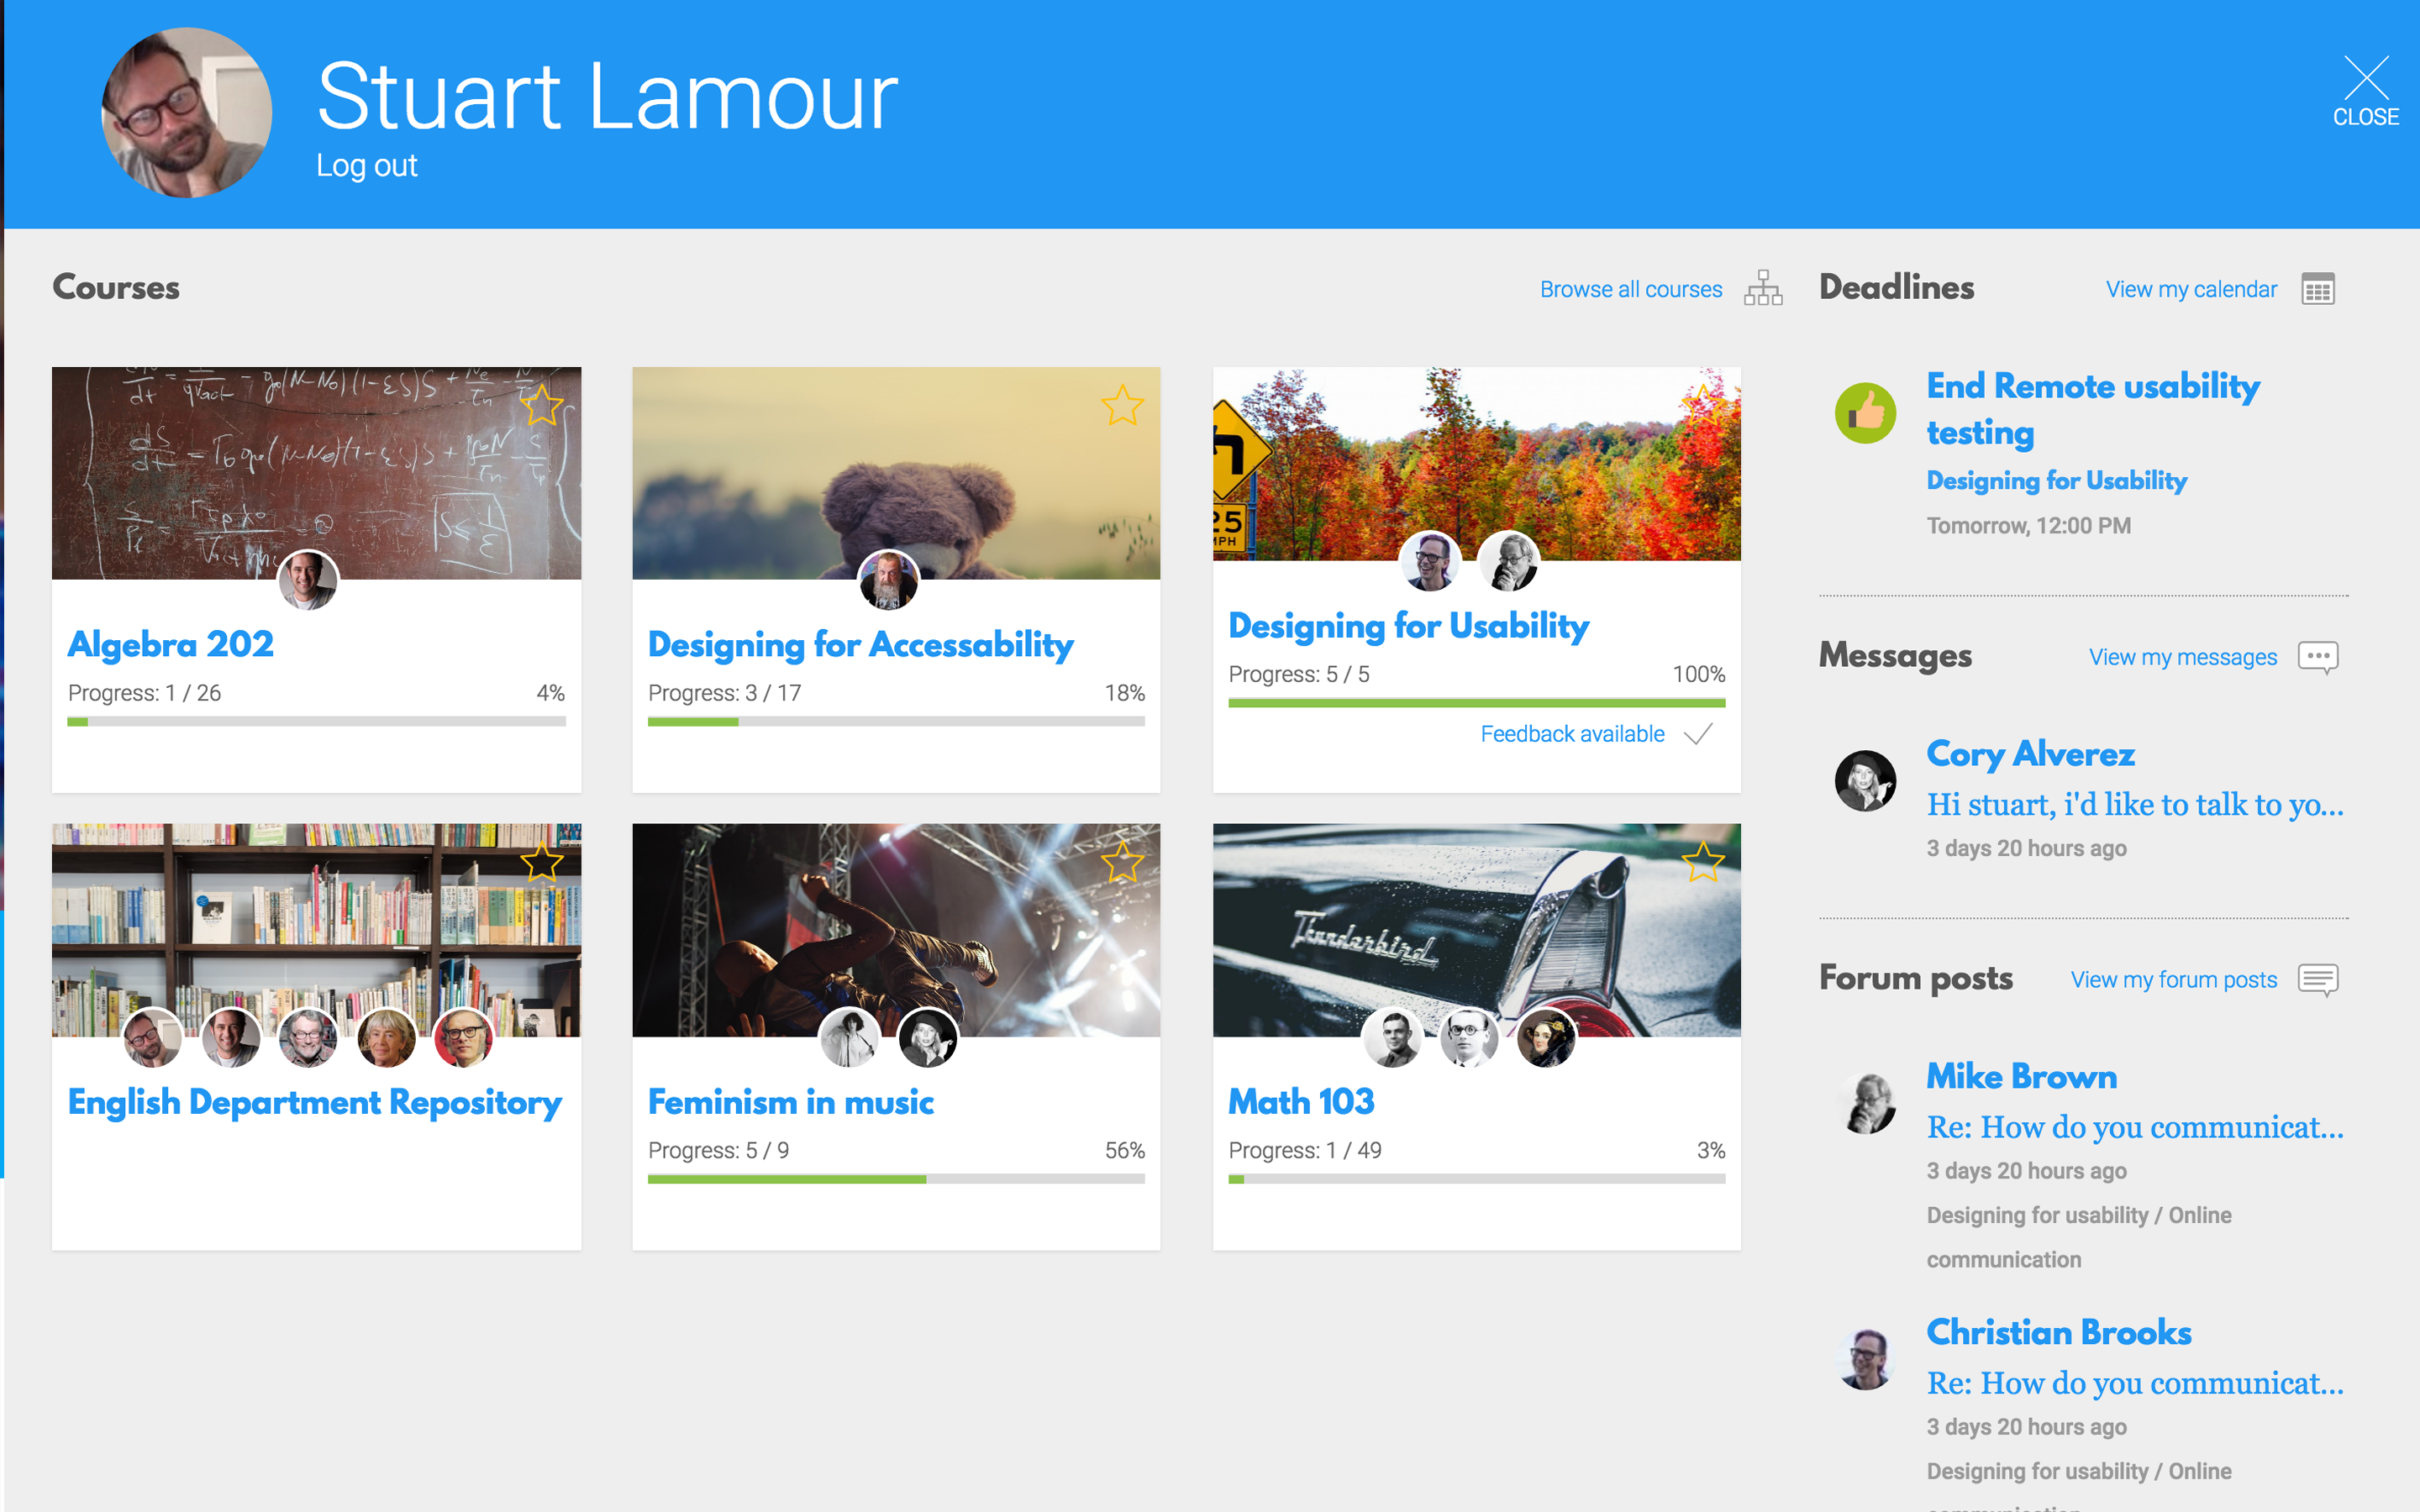
\includegraphics[scale=0.16]{snap-personalmenu.png}  
	\caption[Halaman \textit{Featured Courses}] {Tampilan tema Snap} 
	\label{fig:snap-personal} 
\end{figure} 
\item \textbf{Mata kuliah dan peserta mata kuliah} \\
IDE UNPAR sudah digunakan dalam proses belajar mengajar selama perkuliahan di UNPAR, sehingga IDE UNPAR sudah terisi dengan data dosen-dosen dan mata kuliah yang mereka ajarkan. Beserta dengan data-data tersebut IDE UNPAR juga sudah terisi dengan data-data mahasiswa aktif di UNPAR.
\item \textbf{\textit{Banner} pada halaman utama}
IDE UNPAR menggunakan sebuah korsel untuk menunjukkan nama situs dan pengumuman seperti pada Gambar \ref{fig:korsel-unpar}. Korsel yang digunakan oleh IDE UNPAR adalah bawaan juga dari tema Snap yang digunakan.
\begin{figure}[H] 
	\centering  
	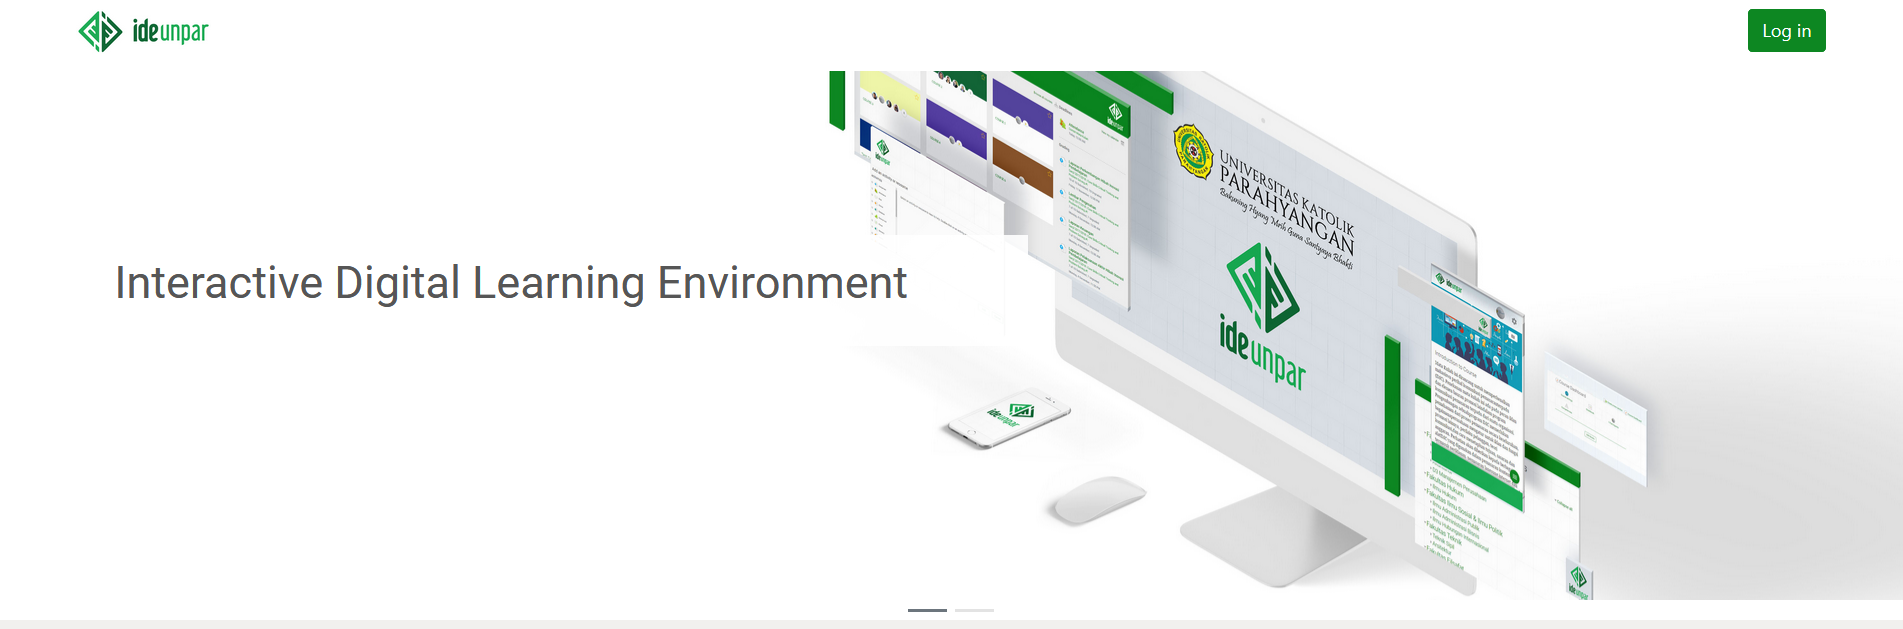
\includegraphics[scale=0.2]{korsel-unpar.png}  
	\caption[Korsel pada halaman utama] {Korsel pada halaman utama IDE UNPAR} 
	\label{fig:korsel-unpar} 
\end{figure}
\item \textbf{Bagian panduan digital} \\
IDE UNPAR juga memiliki bagian untuk petunjuk dan panduan-panduan menggunakan IDE UNPAR, terlihat pada Gambar \ref{fig:panduan-digital}. Bagian ini berisi \textit{courses} Moodle yang terletak dibawah korsel pada halaman utama. Bagian panduan digital IDE UNPAR 
\begin{figure}[H] 
	\centering  
	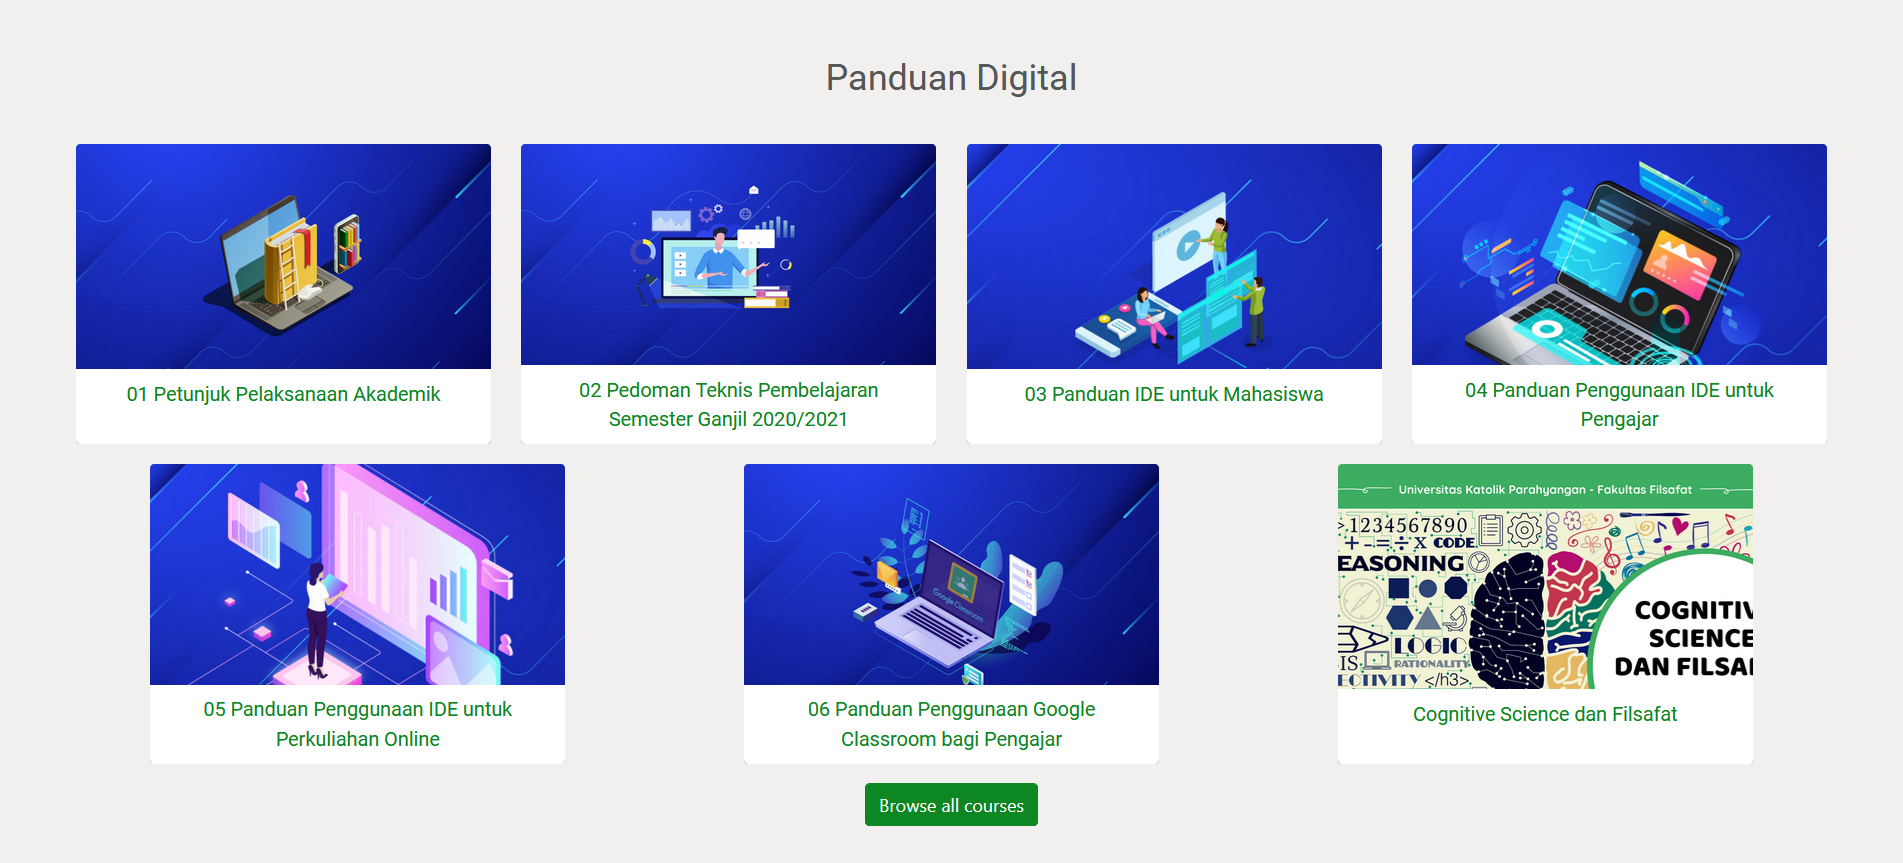
\includegraphics[scale=0.2]{panduan-digital.png}  
	\caption[Bagian panduan digital] {Bagian panduan digital pada halaman utama IDE UNPAR} 
	\label{fig:panduan-digital} 
\end{figure} 
\item \textbf{Video YouTube tersemat} \\
Halaman utama IDE memilik vidio YouTube yang tersemat berjudulkan "Tutorial IDE Mahasiswa".
\item  \textbf{Branding UNPAR} \\
Branding yang dimaksud adalah penggunaan logo IDE UNPAR, nama IDE UNPAR dan skema warna yang berbeda dari skema warna milik Moodle dan skema warna bawaan tema Snap.
\item \textbf{SSO} \\
IDE UNPAR menggunakan SSO UNPAR untuk menangani pengguna yang ingin masuk ke dalam IDE UNPAR. Tombol \textit{login} pada halaman utama akan mengarahkan pengguna ke halaman SSO UNPAR seperti pada Gambar \ref{fig:sso-unpar} untuk memasukkan kredensial mereka.
\begin{figure}[H] 
	\centering  
	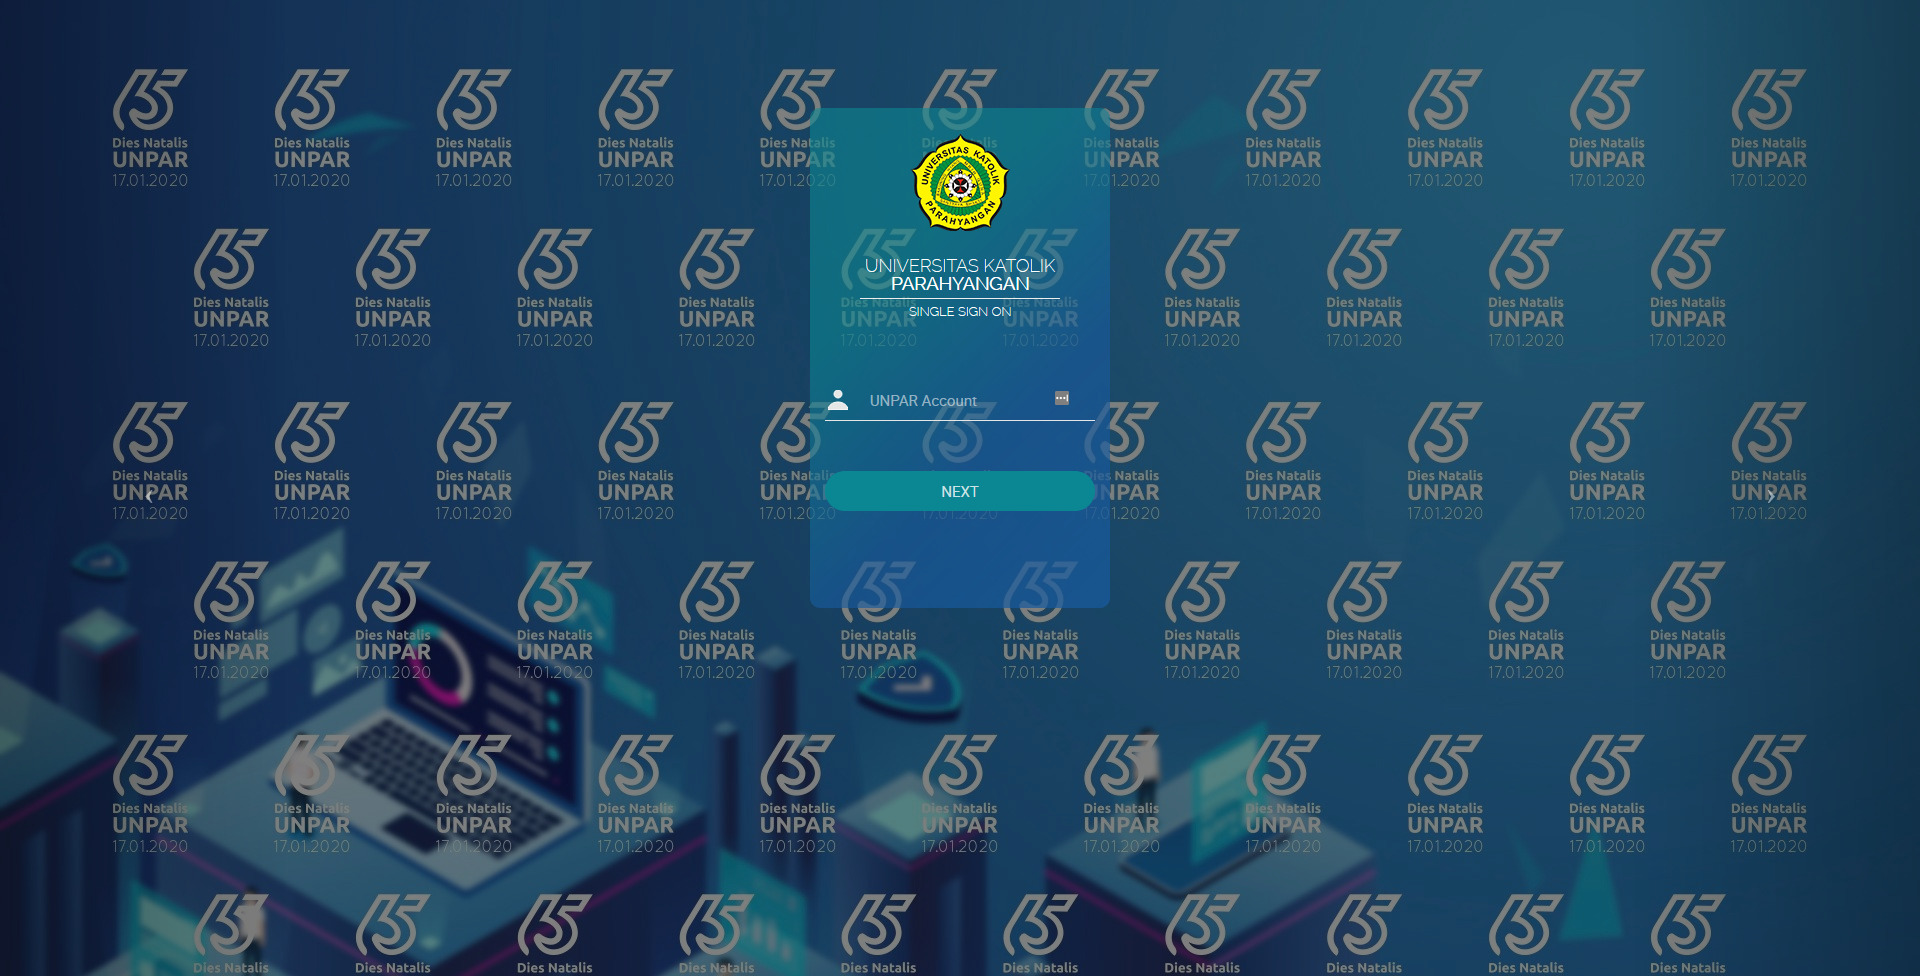
\includegraphics[scale=0.2]{sso-unpar.png}  
	\caption[Halaman SSO UNPAR] {Halaman SSO UNPAR} 
	\label{fig:sso-unpar} 
\end{figure} 


\end{enumerate}

		
		\item \textbf{Menulis dokumen skripsi bab 1, bab 2, bab 3. dan bab 5}\\
		{\bf Status :} Ada sejak rencana kerja skripsi.\\
		{\bf Hasil :} Dokumen skripsi mulai ditulis setelah Moodle mobile dipelajari dan aplikasi Moodle mobile standar dapat dihubungkan dengan situs demo.Dalam dokumen skripsi bab 1 membahas latar belakang, rumusan masalah, tujuan, batasan masalah, metodologi, dab sistematika pembahasan. Bab 2 membahas IDE UNPAR, Moodle, Moodle Mobile,  Moodle mobile \textit{developments}, dan lingkungan pengembangan. Bab 3 membahas Kondisi IDE UNPAR dibandingkan dengan Moodle standar, Moodle demo, Penyesuaian Moodle mobile dengan IDE UNPAR, dan Lisensi Moodle mobile. Bab 5 baru tersisi dengan pembahasan Lingkungan pengembangan peneliti dan Penyesuaian Tema.
		

	\end{enumerate}

\section{Pencapaian Rencana Kerja}
Langkah-langkah kerja yang berhasil diselesaikan dalam Skripsi 1 ini adalah sebagai berikut:
\begin{enumerate}
\item Memplajari Moodle mobile
\item Menganalisa lisensi dari Moodle mobile
\item Menyiapkan lingkungan pengembangan
\item Menulis sebagan dokumen skripsi bab1 , bab 2,  bab 3, dan bab 5
\end{enumerate}




\vspace{1cm}
\centering Bandung, \tanggal\\
\vspace{2cm} 
\includegraphics{Signature}\\ \nama \\ 
\vspace{1cm}

Menyetujui, \\
\ifdefstring{\jumpemb}{2}{
\vspace{1.5cm}
\begin{centering} Menyetujui,\\ \end{centering} \vspace{0.75cm}
\begin{minipage}[b]{0.45\linewidth}
% \centering Bandung, \makebox[0.5cm]{\hrulefill}/\makebox[0.5cm]{\hrulefill}/2013 \\
\vspace{2cm} Nama: \pembA \\ Pembimbing Utama
\end{minipage} \hspace{0.5cm}
\begin{minipage}[b]{0.45\linewidth}
% \centering Bandung, \makebox[0.5cm]{\hrulefill}/\makebox[0.5cm]{\hrulefill}/2013\\
\vspace{2cm} Nama: \pembB \\ Pembimbing Pendamping
\end{minipage}
\vspace{0.5cm}
}{
% \centering Bandung, \makebox[0.5cm]{\hrulefill}/\makebox[0.5cm]{\hrulefill}/2013\\
\vspace{2cm} Nama: \pembA \\ Pembimbing Tunggal
}
\end{document}

